\clearpage

\section{プログラムの仕組みを知ろう}
\subsection{プログラムの流れをあやつろう}

スクリプトに\ruby{旗}{はた}を立てる方法を覚えましょう。旗というのは屋上についてヒラヒラしたり山の\ruby{頂上}{ちょう|じょう}に立ってるものです。スクリプトの旗は\ruby{目印}{め|じるし}になる場所を意味します。自分で好きな名前をつけてスクリプトの中に目印として旗を立てておくことができます。
ファイル→「開く」メニューから「hata.hsp」を読み込みましょう。

\begin{description}
    \item *hata
    \item \ \ redraw 0
    \item \ \ pos 0,0
    \item \ \ mes {\textquotedbl}えっさ{\textquotedbl}
    \item \ \ redraw 
    \item \ \ wait 50
    \item \ \ redraw 0
    \item \ \ pos 0,0
    \item \ \ mes {\textquotedbl}   ほいさ{\textquotedbl}
    \item \ \ redraw 1
    \item \ \ wait 50
    \item \ \ goto *hata
\end{description}

[F5]キーを押して実行すると、「えっさ」と「ほいさ」の文字が\ruby{交互}{こう|ご}に表示されます。
スクリプトの行数は少ないのに、何度もくり返して実行されているのはなぜでしょう。
これが、旗の機能を使った例です。
旗のことをHSPではラベルと呼んでいます。

\begin{description}
    \item (HSPのルール)
\end{description}

\begin{description}
    \item 旗は「*」の後に旗の名前を自由に決めて書くことができる
    \item (ただし命令と同じ名前は使えません)
    \item goto命令は指定したラベル(旗)に飛ぶための命令
    \item gotoの後にスペースに続けて飛び先のラベル(旗)を指定します
    \item goto命令が実行された後は飛び先のラベル(旗)から実行が続けられます
\end{description}

つまり、1行目からスクリプトが実行されていますが、「goto*hata」まで来ると、また「*hata」の行まで戻ってしまいます。
こうして、このスクリプトは、「*hata」の行から「goto*hata」までを\ruby{永遠}{えい|えん}にくり返します。

このようにくり返しにより、\ruby{大量}{たい|りょう}の作業をこなしてしまうのがプログラムの\ruby{凄}{すご}いところです。

\begin{description}
    \item (HSPのルール)
\end{description}

\begin{description}
    \item 「redraw 0」から「redraw 1」は画面を更新するための命令
    \item 画面を\ruby{描}{か}き始める前に「redraw 0」を書いておく
    \item 画面を\ruby{描}{か}き終わったら「redraw 1」を書いておく
\end{description}

自分なりに、mesのメッセージや、wait命令の待ち時間を変更して、どのような結果になるか試してみましょう。

\subsection{\ruby{変数}{へん|すう}と\ruby{計算}{けい|さん}}

プログラミングを覚える上で、とても重要な\ruby{変数}{へん|すう}というものについて覚えていきましょう。
変数はどんなコンピューター言語でも使われている大切な機能です。
どんなものなのか、まずスクリプトを見てみましょう。
ファイル→「開く」メニューから「keisan.hsp」を読み込みましょう。

\begin{description}
    \item \ \ x=100
    \item \ \ pos 20,120
    \item \ \ color 0,0,255
    \item \ \ mes {\textquotedbl}こたえは{\textquotedbl}+x
\end{description}

実行すると、画面の中央上に「こたえは100」が表示されましたね。
mes命令の”こたえは”の後ろに「+x」が付けられています。ここに出て来る「x」が「変数」です。

\begin{figure}[H]
    \begin{center}
        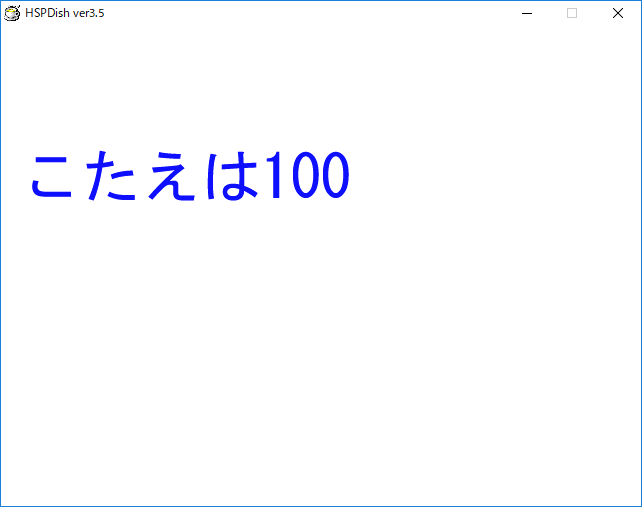
\includegraphics[keepaspectratio,width=7.382cm,height=5.831cm]{text02-img/text02-img044.png}
        \caption{keisan.hspの実行画面}
    \end{center}
\end{figure}

変数はよく、「いれもの」にたとえられます。数値をきおくしておく、「いれもの」です。
「いれもの」には名前をつけることができます。たとえば「x」という名前の「いれもの」に数値を入れておくには、「x=100」のように書きます。

\begin{figure}[H]
    \begin{center}
        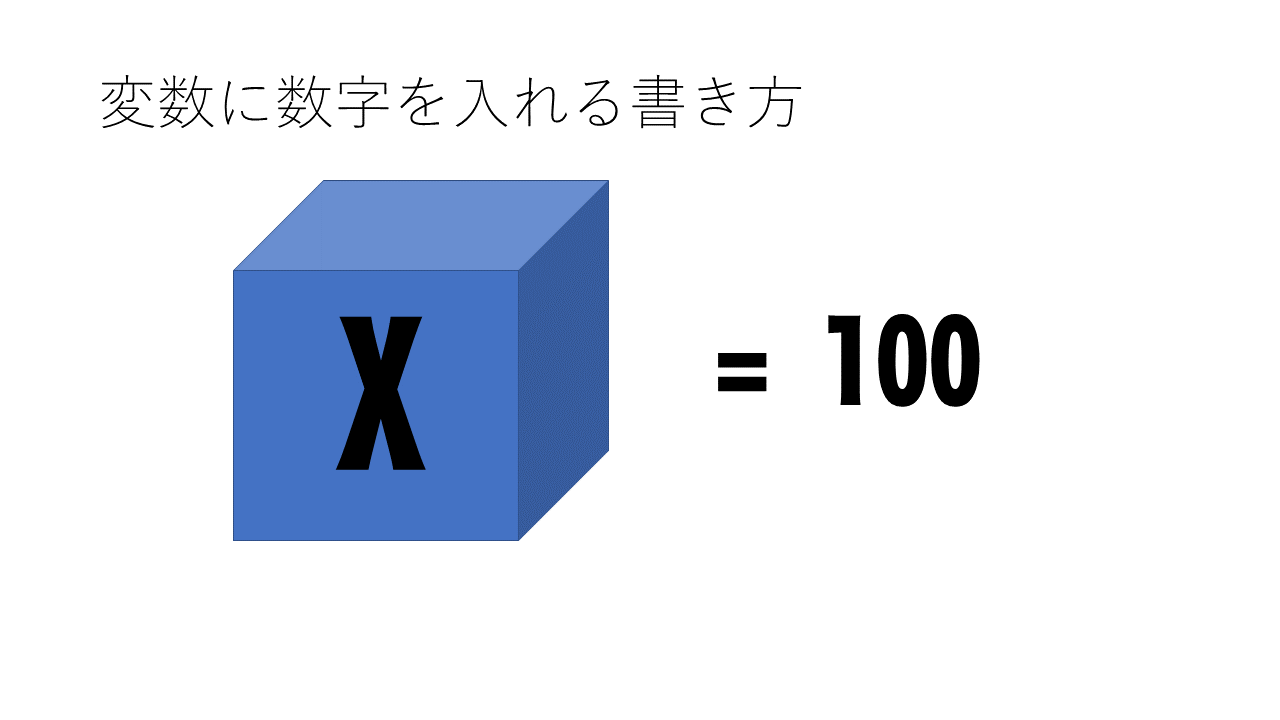
\includegraphics[keepaspectratio,width=10.478cm,height=5.106cm]{text02-img/text02-img045.png}
    \end{center}
\end{figure}

このスクリプトではxという名前をつけてあります。これを変数xと呼びます。(名前は1文字でなく長い名前でもかまいません。日本語でもいいです。でも打ち込みやすいので1文字でもよく使われます)
名前は命令と同じものは使えないので注意しましょう。

「x=100」でxという名前の変数に100という数値が入ります。これを「代入」と呼んでいます。変数に数値を入れておくと命令で指定するパラメーターとして指定することができるようになります。
つまり「pos 100,120」を、「pos x,120」と書くこともできるのです。

\begin{description}
    \item (HSPのルール)
\end{description}

\begin{description}
    \item 「変数の名前=数値」で変数に値を入れることができる(代入)
    \item 変数に数値を入れておくとパラメーターとして使える
    \item mes命令の中で「+変数」を書くことで変数の中身を表示できる
\end{description}

変数に値を代入しておくことで同じ数値を指定する部分をまとめて変更したり、命令と別な場所で指定をすることができるようになります。

ほかにも、数値を書く部分に記号を入れて計算をすることができます。
計算は\ruby{電卓}{でん|たく}などで使われている\ruby{四則演算}{し|そく|えん|ざん}が基本になります。

\begin{figure}[H]
    \begin{center}
        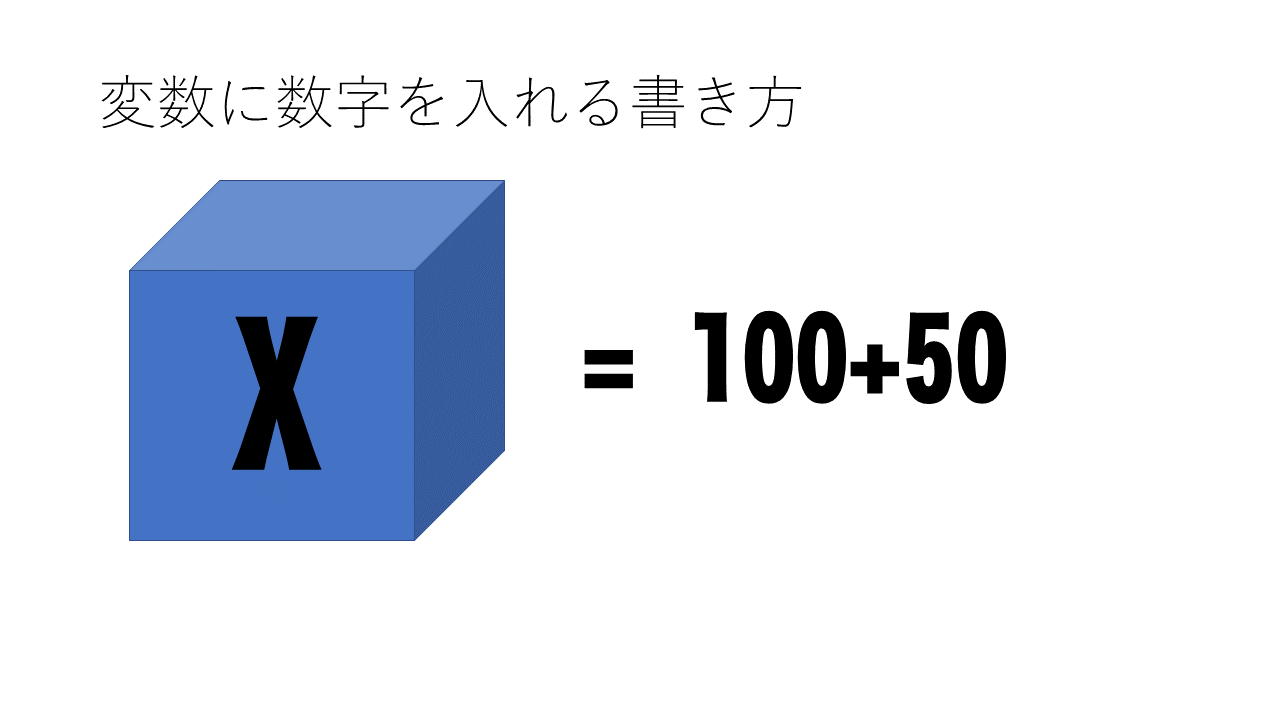
\includegraphics[keepaspectratio,width=11.695cm,height=5.741cm]{text02-img/text02-img046.png}
    \end{center}
\end{figure}

\begin{description}
    \item (HSPのルール)
\end{description}

\begin{description}
    \item 数式とは、数値と変数、またはそれらを\ruby{計算式}{けい|さん|しき}でつなげて書くこと
    \item 「+」は\ruby{足}{た}し\ruby{算}{ざん}、「-」は\ruby{引}{ひ}き算、「*」は\ruby{掛}{か}け算(×)、「/」は\ruby{割}{わ}り算(÷) 
\end{description}

数式とはつまり、数値を指定する場所に1+1と書いたら2を書いたのと同じことになる、ということです。(コンピューターですから計算は\ruby{大}{だい}の\ruby{得意}{とく|い}です)
つまり、「x=100+20」は「x=120」と同じことになるのです。
変数と計算で何ができるのか、まだよくわからない人も多いと思いますが、あわてずにゆっくり覚えるようにしましょう。

\subsection{\ruby{乱数}{らん|すう}を使ってみよう}

変数を使った例をもう1つ紹介します。ファイル→「開く」メニューから「stars.hsp」を読み込みましょう。100個の「☆」をmes命令で画面に表示しています。
ここでは、「☆」を表示する位置をバラバラにするために\ruby{乱数}{らん|すう}を使用しています。
乱数は、ゲームなどでよく使われている要素の1つで、コンピューターが選んだバラバラな数字を作るものです。
バラバラな数字は、決められた数字の\ruby{範囲}{はん|い}で作ることができ、何が出るかはだれにも\ruby{予想}{よ|そう}ができません。

\begin{figure}[H]
    \begin{center}
        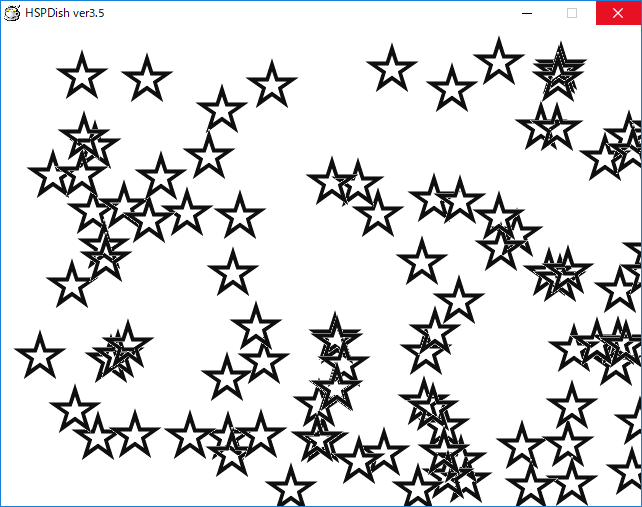
\includegraphics[keepaspectratio,width=7.99cm,height=6.297cm]{text02-img/text02-img047.png}
        \caption{stars.hspの実行画面}
    \end{center}
\end{figure}

スクリプトを見てみましょう。

\begin{description}
    \item \ \ repeat 100
    \item \ \ x=rnd(640)
    \item \ \ y=rnd(480)
    \item \ \ pos x,y
    \item \ \ mes {\textquotedbl}☆{\textquotedbl}
    \item \ \ loop
\end{description}

変数xと変数yは、pos命令で「☆」を表示する位置をきおくするものとして使われています。
「x=rnd(640)」は、0〜639(640通り)までのバラバラな数字を変数xに代入します。このような書き方を「\ruby{関数}{かん|すう}」と呼んでいます。

\begin{figure}[H]
    \begin{center}
        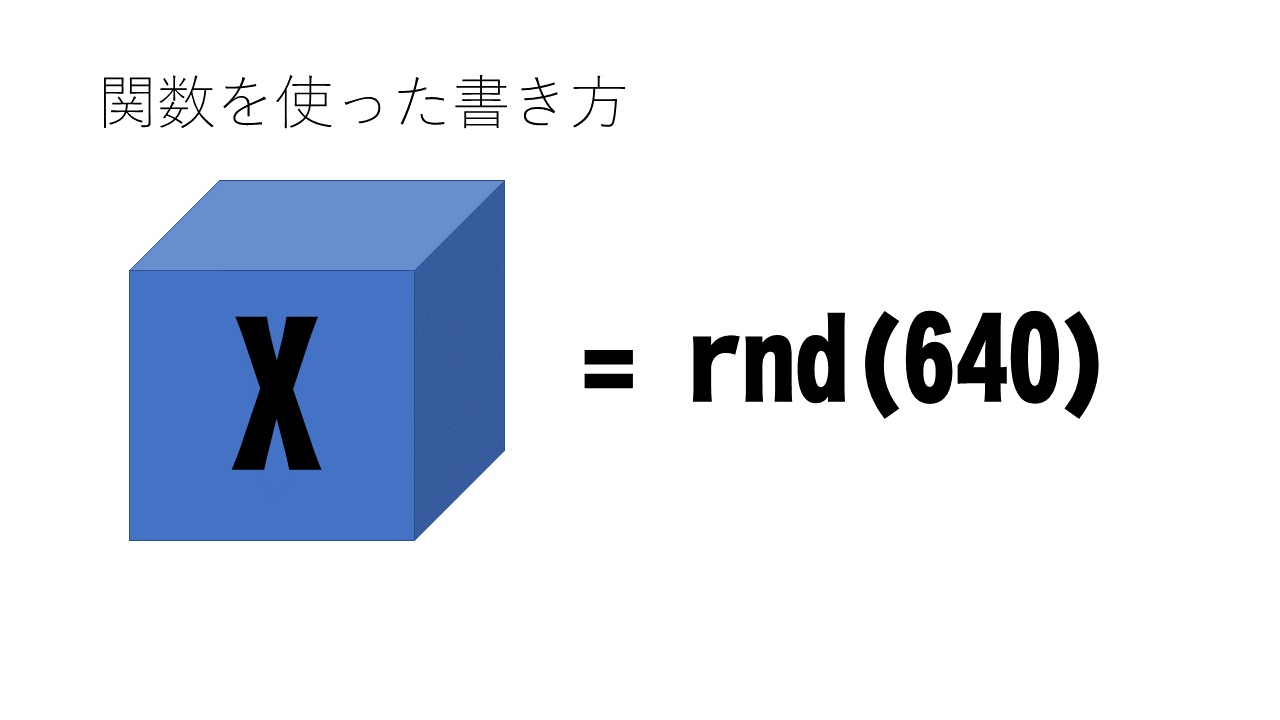
\includegraphics[keepaspectratio,width=11.906cm,height=5.662cm]{text02-img/text02-img048.png}
    \end{center}
\end{figure}

\begin{description}
    \item (HSPのルール)
\end{description}

\begin{description}
    \item 「変数=rnd(乱数の最大値)」でバラバラな数字を得ることができる
    \item 関数は、「変数=関数(パラメーター)」という書き方で使うことができる
\end{description}

「y=rnd(480)」も同様に0〜479までの数字を代入します。画面のサイズが、横640、縦480ですから、画面上のでたらめな位置をpos命令で指定することができます。
repeat命令で100個の「☆」を描いていますが、この数字を変えたり(あまり大きな数字にすると遅くなるので注意してください)、乱数の範囲を変えてみながら、どのように画面が変化するか確認してみましょう。
\ruby{余裕}{よ|ゆう}のある人は、でたらめな色で「☆」をたくさん表示する方法を考えてみてください。

\subsection{\ruby{条件判断}{じょう|けん|はん|だん}とは}

変数と数字を使って計算ができることはわかりました。さらにもう1つ、\ruby{重要}{じゅう|よう}な\ruby{要素}{よう|そ}として「条件判断」を覚えることができれば、プログラミングの大きな\ruby{関門}{かん|もん}を1つこえることになります。
それほど、「条件判断」はプログラミングの大きな要素であり、「条件判断」なしでは大きなプログラムを作ることはできません。

\begin{figure}[H]
    \begin{center}
        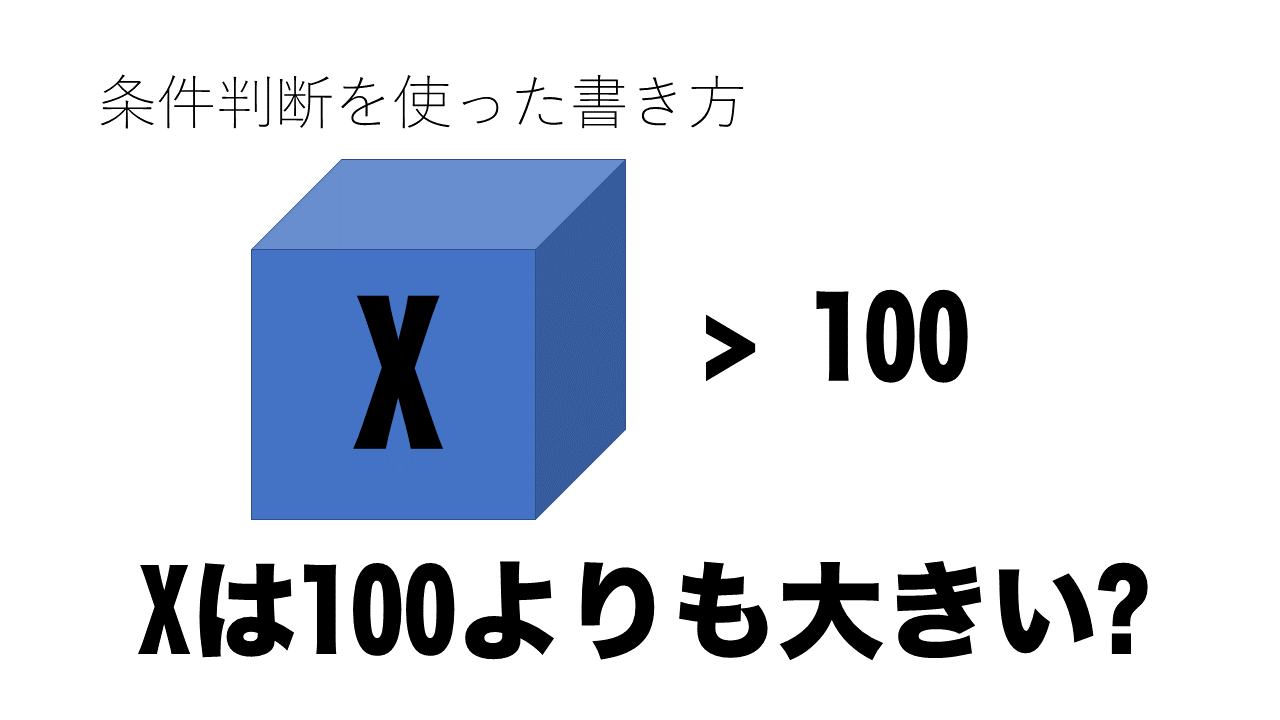
\includegraphics[keepaspectratio,width=12.33cm,height=6.939cm]{text02-img/text02-img049.png}
    \end{center}
\end{figure}

\begin{description}
    \item (HSPのルール)
\end{description}

\begin{description}
    \item if命令により条件を判断することができる
    \item ifの後にスペースに続けて条件式を指定します
    \item その後で「:」に続けて条件が正しい時に実行される命令を書きます
\end{description}

\begin{description}
    \item (条件式はいくつか書き方があります)
\end{description}

\begin{description}
    \item \ \ 条件式 \ \ \ \ \ \ \ \ \ 意味
    \item \ \ {}-{}-{}-{}-{}-{}-{}-{}-{}-{}-{}-{}-{}-{}-{}-{}-{}-{}-{}-{}-{}-{}-{}-{}-{}-{}-{}-{}-{}-{}-{}-{}-{}-{}-{}-{}-{}-{}-{}-{}-{}-{}-{}-{}-{}-{}-{}-{}-{}-{}-{}-{}-
    \item \ \ 変数名 = 数値\ \ 変数の内容と数値が同じである
    \item \ \ 変数名 ! 数値\ \ 変数の内容と数値が同じではない
    \item \ \ 変数名 {\textless} 数値\ \ 変数の内容より数値の方が数が大きい
    \item \ \ 変数名 {\textgreater} 数値\ \ 変数の内容より数値の方が数が小さい
\end{description}

たとえば、

\begin{description}
    \item if a=0 : mes “0です”
\end{description}

という行は、変数aの内容が0だった時に「0です」というメッセージを出すという意味になります。

条件判断と変数を使うことで、とても複雑な動作を作ることができます。

最初は、想像がつきにくいかもしれませんが、スクリプトがどのように動いて判断されるのかを、頭の中でゆっくり考えてみてください。

スクリプトの書き方は、もちろんここで説明したことがすべてではありません。しかし、ここに書かれている基本を押さえておけば、誰でもある程度のソフトまでは作ることができるはずです。そして、さらにステップアップをしたい人は、HSPのスクリプトのすべてが書かれている、マニュアルや、本を読んでみてください。決してあせらないで、自分にできる範囲でスクリプトを組んでいきましょう。

これまで説明してきたことの多く、変数やラベルといったものは、
他のプログラミング言語、とりわけBASICと呼ばれているものに近いです。HSPで初めてプログラム
について知ったという人が、他の言語を覚える時が来ても、HSPで知ったことが役に立つに違いありません。

\subsection{例題に挑戦しよう}

ここまで終わってしまった人は、以下の例題にも挑戦してみよう。

\begin{itemize}
    \item 動きのある画面を作ってみる
    \item 条件判断を自分で使ってみよう
    \item くり返しの方法を知ろう
    \item ポーカーゲームで遊んでみよう
    \item スイッチを使ったゲームで遊んでみよう
\end{itemize}

例題の考え方がわからない時は、近くのTAか先生に聞いてください。
わからない所は、そのままにせず、必ず答えを見つけてから先に進みましょう。

